\section{Introduction}
\label{sec:intro}
Microblogging has taken over the Internet as one of the most
popular forms of online social networking.
Twitter \cite{website:Twitter},
or the Chinese equivalent,
Sina Weibo \cite{website:Sina}, allows users
to instantly broadcast short messages of up to 140 characters
with optional images and other meta data to all their followers.
Such messages maybe reposted with or without
comments by the followers and thus get transmitted throughout the social network.
%very rapidly, sometimes described as being ``viral''.
Many of the microblogs carry unconfirmed and uncertain information,
and when they get spread around quickly,
they become rumors.

There is no uniform definition of rumors according to social scientists.
In our work, a {\em rumor} is defined as an unverified or unconfirmed statement or
report circulating in a community \cite{website:OxfordDic}.
%a widely circulated statement
%about an object, event or issue, which is inconsistent with
%facts or known scientific evidences.
%A {\em non-rumor} is any other original message which is not a rumor.
By this definition, a stand-alone microblog which has
not been spread around is not a rumor.
%We are instead interested in the message as well as its propagation behavior.
Breaking news such as celebrity getting married that gets spread wildly online
is not a rumor either, because it is factual information.
Discussions about personality by horoscope signs
are considered rumors because there is no way to confirm their
truthfulness. Some rumors eventually are verified to be false;
these are called {\em false rumors} in this paper.
These rumors are created either intentionally or unintentionally,
but carry false or even malicious information and spread widely
in the community. For instance, some ``urban legends'' such as
``Coke can dissolve a tooth overnight'' are considered
false rumors here because they are spread widely in the community
and proven to be false eventually.
Recent past has witnessed many incidents of
online false rumors causing massive public panic and social unrest.
On April 23, 2013, a false rumor on Twitter about an explosion in
Whitehouse injurying President Obama sent the Dow down
140 points within a few minutes.
In March, 2011, after the Japanese Fukushima nuclear disaster, a
Sina Weibo post claimed that increased consumption of iodized salt
can protect human from
nuclear radiation and this message caused millions of
people to raid the supermarkets around China to buy salt
and even soy sauce.
%Because social
%networks have been one of the primary sources of information for many
%online users, excessive transmission of rumors can shake public confidence
%of the microblogging service and hurt this industry in general.
%Moreover, some ill-motivated rumors have severe consequences such as
%public fear, social unrest or even man-made disasters.
%Due to the large scale and fast nature of internet rumors,
Because of these and many other similar damaging incidents,
automatic detection of false rumors on social network has
recently gathered substantial research interest and
is also the goal of this paper.

While some researchers have worked previously on
Twitter (see \secref{sec:related}),
%\cite{ratkiewicz2010detecting,qazvinian2011rumor,mendoza2010twitter,castillo2011information,umejima2011tendency,jin2013epidemiological,okazaki2013extracting},
this paper focuses on false rumor detection on
Sina Weibo, for which only limited research has been done
\cite{yang2012automatic,sun2013detecting,bao2013new}.
Automatic detection of false rumors is generally a hard problem, because
without proper background knowledge or concrete,
official evidence against, even human being cannot distinguish
between the false rumor and other messages.
%
%Automatic detection of rumors on microblogging network is a hard problem
%because and has only recently been attempted for Twitter.
%Sina Weibo is widely used by human beings as a popular social networking platforms in China.
%Sina weibo is a Twitter-like microblogging service.
%Compared with traditional media like newspaper and television, Weibo is more timeous for news propagation.
%However, because verification of the authenticity of messages is lacking, there is plenty of misinformation in Weibo.
%The most representative one is rumor.
%
%Mostly, rumors are hard to recognize because they are confused with truth.

\begin{figure}[th]
%\setlength{\abovecaptionskip}{10pt}
%\setlength{\belowcaptionskip}{5pt}
\centering
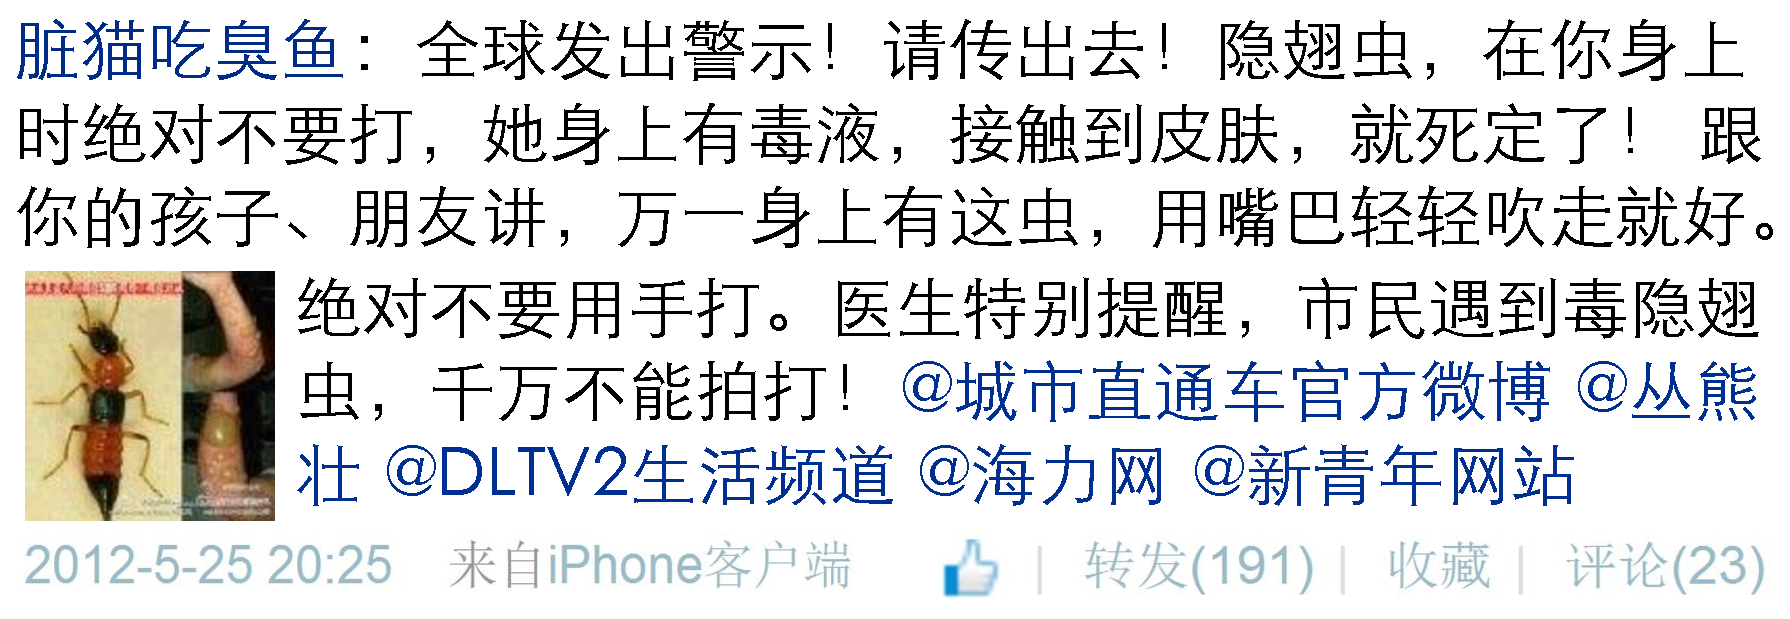
\epsfig{file=example1.eps, width=0.9\columnwidth}
\caption{False rumor about Rove Beetle}
\label{fig:beetle-rumor}
\vspace*{2mm}
%\setlength{\belowcaptionskip}{0pt}
\epsfig{file=example2.eps, width=0.9\columnwidth}
\caption{Normal message about Rove Beetle}
\label{fig:beetle-truth}
\end{figure}

Consider the following two postings from Sina Weibo (translated from
the original messages in \figref{fig:beetle-rumor} and \figref{fig:beetle-truth}):
\begin{itemize}
\small
\item {\bf Dirty Cat Eats Foul Fish}: \textit{Global warning! Please repost!
You should never crush a rove beetle if it lands on your skin.
Rove beetles contain venom which kills people for sure if it 
contacts skin! Tell your children and friends that it's better
to just gently blow the rove beetle away if it lands on your skin. 
Doctors specially warn that if you come across
a rove beetle, never smash it with hands! @AccessCity @CongXiongzhuang
@DLTVLivingChannel @hiliziWebsite @NewYouthWeb}
\item {\bf Wenzhou City News}: \textit{[Don't crush this beetle with 
hands when you see it] Rove beetles have been discovered
in a school of Wenzhou. According to a doctor, rove beetle doesn't bite
human beings, but once the venom in its body comes in contact with human skin,
it can quickly cause blistering and festering, spreading to other areas and
getting worse if you scratch it. 
If you ever touch the venom of rove beetle, please clean the skin repeatedly
with soap water, 4\% baking soda solution or 10\% ammonia, and seek help at
a local hospital immediately.}
\end{itemize}

Both messages quote the words of doctors, include vivid photos,
and have comparable number of reposts, which makes them
hardly distinguishable. The first message even {\em mentioned}
a few prominent organizational
users with the ``@'' sign, which appears to be official.
However, the first posting is a false rumor while the second is not.
The truth is, venom of rove beetle does not kill people but can result in
skin infection. Such knowledge is hard to come by for average
people, which explains why some innocent people repost false rumors and
inadvertently help their spread. The detection task is even
harder for computers, because the two messages contain very similar
keywords such as ``rove beetle'', ``crush'', ``venom'', ``skin''
and ``doctor''. Existing natural language processing techniques can easily
confuse the two messages due to their similarities.

\begin{figure*}[th]
\centering
\epsfig{file=example1_details.eps, width=2\columnwidth}
\caption{Fragment of false rumor propagation graph}
\label{fig:example1_details}
\vspace*{2mm}
\epsfig{file=example2_details.eps, width=1.4\columnwidth}
\caption{Fragment of normal message propagation graph}
\label{fig:example2_details}
\end{figure*}

One way to understand the difference between these two messages
is by looking at the message propagation structures.
\figref{fig:example1_details} and
\figref{fig:example2_details} illustrate the initial parts of the
propagation graphs for the above examples.
Each node in the graph (denoted by rounded box) represents either
an {\em opinion leader} or
a {\em normal user}. We will define {\em opinion leader}
and {\em normal user} in \ref{sec:tree}. Each node
includes the username and his or her message (either the original message
or the repost message). Furthermore,
the node for an opinion leader also carries the number of followers
and friends, number of reposts. It can be seen that the
false rumor (\figref{fig:example1_details}) is first posted by
a normal user, then reposted and supported by some opinion leaders
and finally reposted by a large number of normal users.
On the contrary, the normal message (\figref{fig:example2_details})
is posted by an opinion leader and reposted directly by many normal users.
This subtle difference of propagation structure is the primary
inspiration of this paper. Besides the overall propagation structure, there
are other hints in \figref{fig:example1_details} that suggest it is a false
rumor: some normal users expressed their doubts or dispproval in their
responses (highlighed in red color). Such signals can be picked up
by high level semantic analysis of each individial response.

Much of the  previous work on false rumor detection focuses
on extracting large number of lexical and semantic features
from the original message and
responses, and learn a model from labeled data
\cite{castillo2011information,qazvinian2011rumor}.
While they do consider the relationships among a thread
of messages, they limit themselves to a flat summary of statistics about
the message propagation patterns, such as the total number of reposts,
depths and degrees of the propagation tree, etc.
They do this for the convenience
of constructing feature vectors for machine learning.
Such an approach is over-simplistic because it ignores the internal
graphical structure of the message transmission as well as the
differences among the users along that structure. Our key insight is
that most false rumors can be identified not only by what the
false rumor says,
but also by the way people respond to it and who these people are.
The propagation patterns, combined with the topics of the thread
and the sentiment of the responses, can give strong
indications whether the original message is the truth or fiction.

%But features coming from one message is always limited. In this paper,
%we take a more holistic approach by considering features from not only the
%original message, but also the reposting messages and responses, the message
%propagation pattern as well as the profile of the users involved.
%The key insight is that while the system may not contain all the knowledge
%required to bust a rumor, the power of the people should not be neglected.
%Most of the rumors can be detected by the way people respond to it
%and who these people are. The propagation patterns, combined with the topic
%of the message and the sentiment of the responses, can give indications of
%whether the original message is the truth or fiction.
%
%Rumors are confusing and prevent people from getting useful information. Besides, if there were many rumors, people may not trust information from Weibo anymore, which is harmful for development of Sina Weibo.
%
%Unfortunately, there are plenty of rumors in Weibo so that Sina Weibo set up a official organization to publish rumors (http://service.account.weibo.com/).
%Why rumors propagate so popularly?  Here is the common pattern how a message is propagated in Sina Weibo. First, one user post a message about something.
%Then, other users who follow him will see this message and they can make comments about it.
%If these users want to share this message with their followers, they will repost the message so that their followers will see this message as well. It likes a propagation tree, the root is the user that post the original message, the second level is the users who follow the root and repost the message. As one message propagate widely, it propagate quickly. In this process, there is no verification of the authenticity of the message. So one rumor will be very popular as long as it is attractive. However, it is impossible to verify all messages and remove rumors in Sina Weibo manually, since people post many messages everyday. Thus it is necessary to detect rumors in Sina Weibo automatically.

%We formulate the rumor detection problem as a classification problem and try to ask computer classify messages to rumor and non-rumor automatically. However, the computer should be smart enough since the rumors are mostly confused with truth.
%Like the examples illustrated above, they both tell us that rove beetle is dangerous and should not squash them but blow them away. However, the rumor (see figure \ref{fig:1}) said it will kill people and the truth {see figure \ref{fig:2}} is it will just result in dermatitis. In this case it is hard for human beings to distinguish them unless they are entomologist or they google it. It is hard for computer to classify them either. The computer must understand the tiny difference between the two messages precisely. Besides, the computer must have the knowledge about the topic, which is impossible because the topic of rumors is various. Moreover, there are some knowledge like news which can not be prestored into computer.
%
%Fortunately, there is not just the content of message but other information that computer could utilize to detect rumors.
%Like the examples illustrated above, the messages are similar as well as original users (they are both verified user with many followers). It prompts us there is some work we could do to improve the performance, which is the propagation features of the message.
%
%In this work, we aim to build a classifier that can classify messages in Sina Weibo automatically.
%Given a message and its reposts, we first build a propagation tree to describe the relationship of reposting.
%Then random walk graph kernel is used to calculate the similarity of two trees. Next, we extract some features
%based on some natural language process methods like word segmentation and sentiment analysis to help identify rumors.
%At last, we combine graph kernel and radial basis function kernel together to build an SVM classifier.

The main contributions of this paper are summarized below:
\begin{itemize}
\item  We model the pattern of message propagation as a tree, which
not only reflects the relation among reposts and their authors but also
the temporal behavior and the sentiment of reposts. The tree can be
simplified to adapt to the space and time requirement of the system
(\secref{sec:tree}).
\item  We propose a random walk graph kernel to model the similarity of
propagation trees. Results suggest that the propagation of false rumors
can be distinguished from other messages (\secref{sec:random}).
%\item  We propose some new features to classify rumors and non-rumors. These features are demonstrated superior
%effectiveness over the features proposed in previous work.
\item  We combine the graph kernel and a radial basis function kernel,
together with other novel features to build a hybrid SVM classifier
(\secref{sec:feature} and \secref{sec:combined}).
Our experiments show the hybrid model achieves significant better
classification accuracy of 91.3\% than those reported in
previous work and can be used for the early detection of false rumors
(\secref{sec:exper}).
\end{itemize}
